\chapter{System Design}
\label{ch:design}

\section{System Architecture}
\label{sec:architecture}
\begin{figure}[H]
\centering
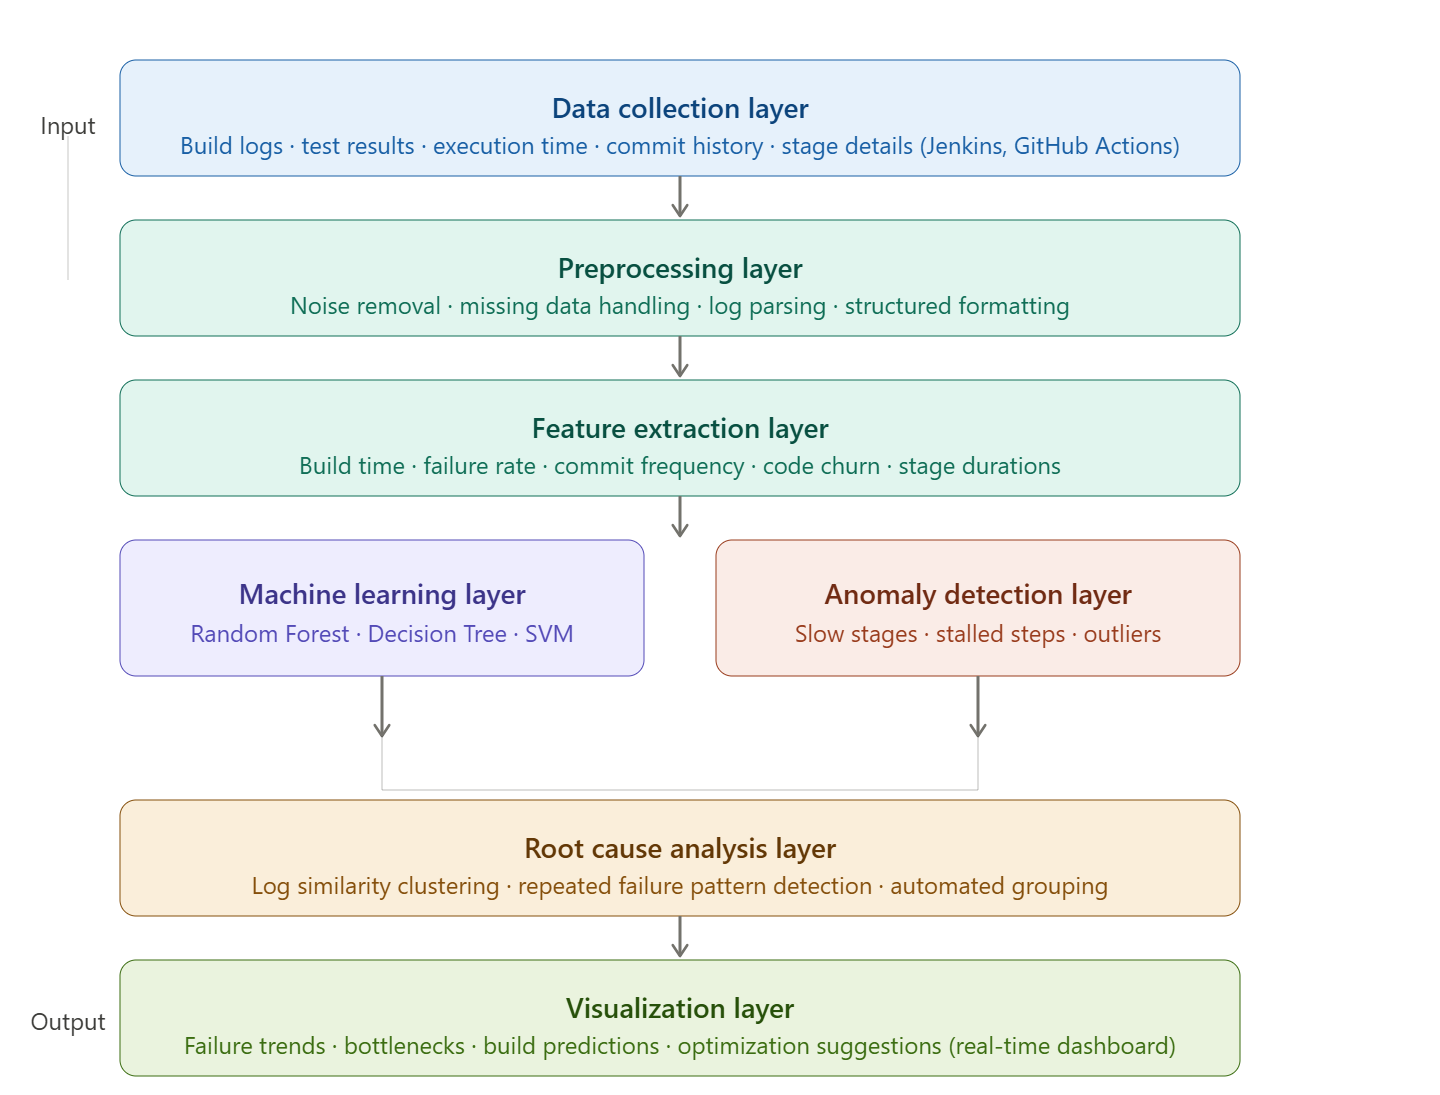
\includegraphics[width=0.92\textwidth]{fig_architecture.png}
\caption{System architecture of the proposed CI/CD optimization framework}
\label{fig:arch}
\end{figure}

The framework uses a modular architecture that analyzes and optimizes CI/CD pipelines through several processing layers (Fig~\ref{fig:arch}). Chapter~\ref{ch:impl} describes how each layer was implemented.
\begin{itemize}
\item \textbf{Data Collection Layer:} Collects historical CI/CD data, including build outcomes, logs, test results, execution times, commit history and job details. The sources are the TravisTorrent export of Travis~CI and the GitHub Actions API. Live data arrives through signed GitHub Actions webhooks, and a Jenkins notification endpoint is also provided.
\item \textbf{Preprocessing Layer:} Cleans and structures the data. It collapses Travis~CI jobs into builds, removes duplicates and re-run attempts, sanitizes logs, and, crucially, enforces when each piece of information becomes available.
\item \textbf{Feature Extraction Layer:} Extracts the size of each change, timing, and the failure history of the repository and of the build's own branch or pull request (its \emph{stream}), using only builds that had finished before the current build started.
\item \textbf{Machine Learning Layer:} Random Forest, Decision Tree and Support Vector Machine were trained as planned, alongside XGBoost, LightGBM and a stacking ensemble. The final model, \tierE, blends a LightGBM classifier with a LightGBM learning-to-rank model.
\item \textbf{Anomaly Detection Layer:} Detects jobs that run abnormally long compared with their own history, and unusual input profiles (Isolation Forest).
\item \textbf{Root Cause Analysis Layer:} Groups similar failure logs (TF-IDF and k-means) and diagnoses failed-job logs with ordered rules, mapping each failure type to a suggestion.
\item \textbf{Visualization Layer:} Displays predictions, alerts, failure trends, bottlenecks, explanations and suggestions on a React dashboard.
\end{itemize}

\section{Proposed Methodology}
\label{sec:methodology}
\begin{figure}[H]
\centering
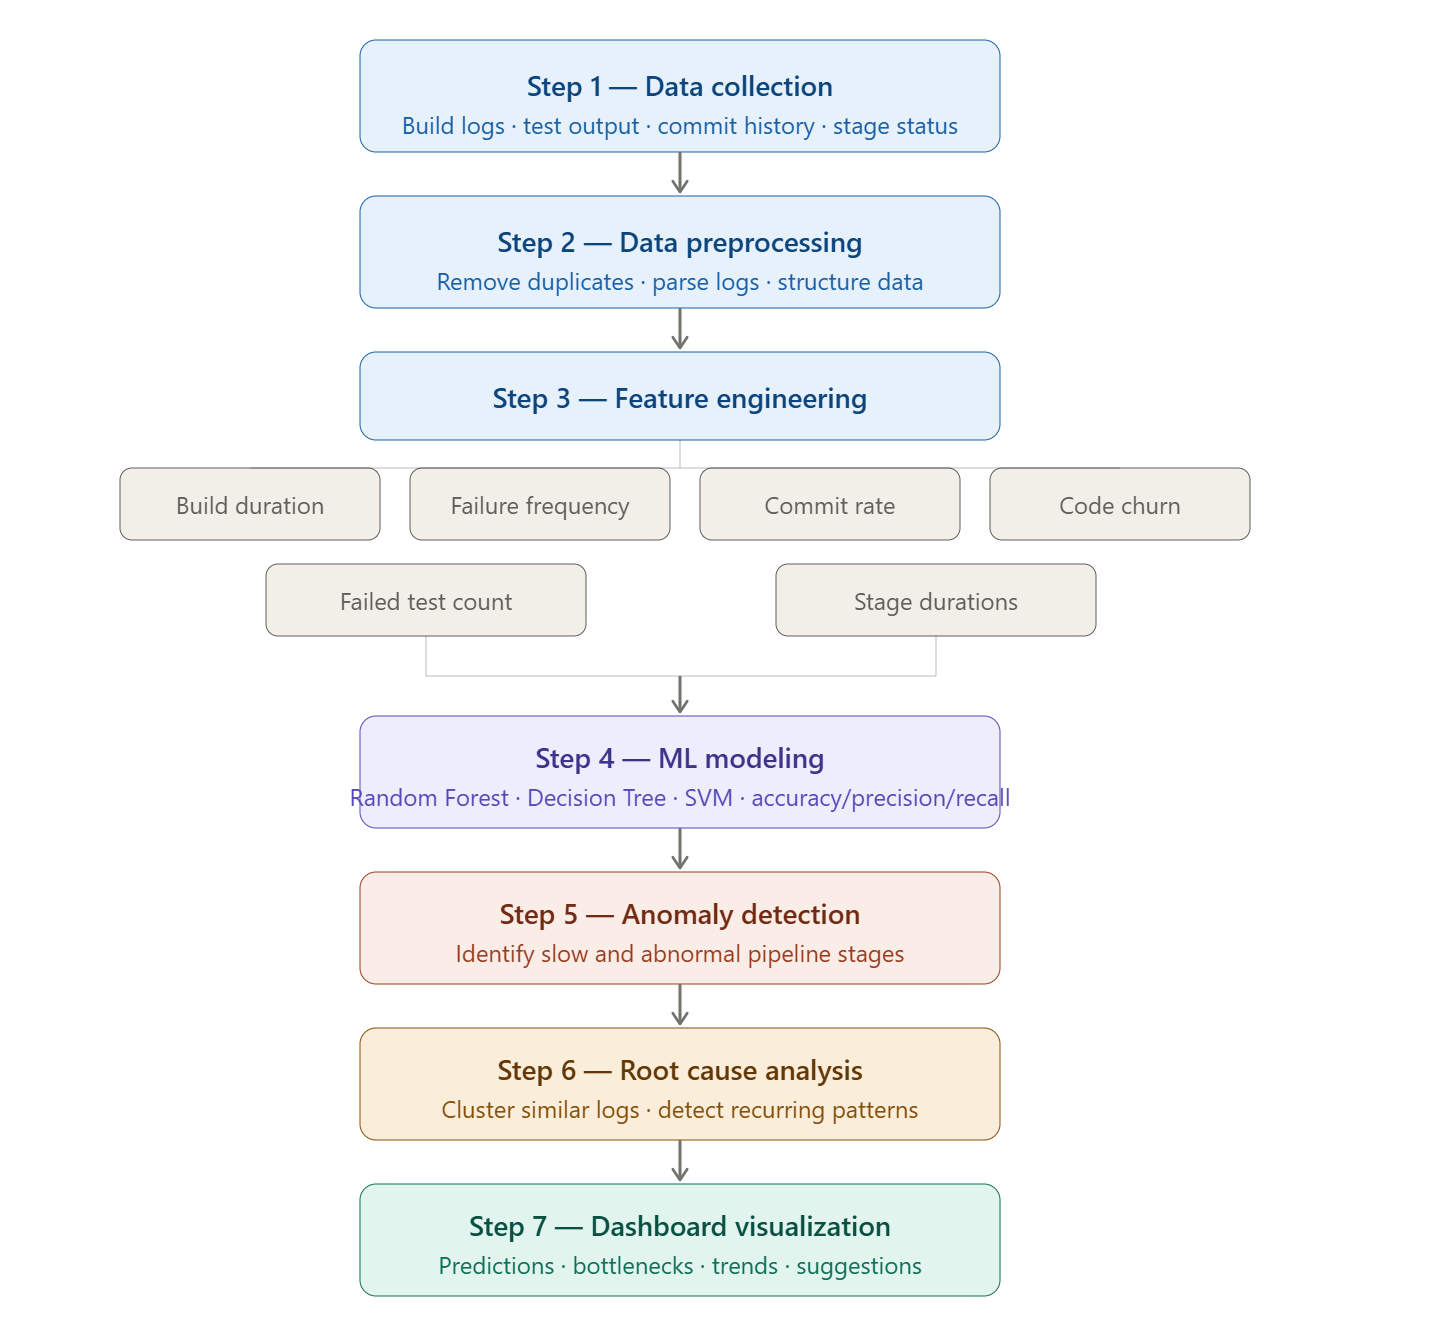
\includegraphics[width=0.78\textwidth]{fig_methodology.png}
\caption{Proposed methodology for AI-driven CI/CD pipeline optimization}
\label{fig:method}
\end{figure}

The solution follows a step-by-step methodology (Fig~\ref{fig:method}): data collection, preprocessing, feature extraction, training of predictive models, bottleneck detection, root cause analysis, and visual dashboard recommendations.

\minorhead{Step 1: Data Collection}
Historical CI/CD data is obtained from TravisTorrent (858,368 Travis~CI builds) and from the GitHub Actions API: workflow runs, their commits, and job timings for 60 public repositories. Live GitHub Actions events arrive through webhooks.

\minorhead{Step 2: Data Preprocessing}
The data is converted to a structured form: jobs are collapsed into builds, duplicates and re-run attempts are removed, unknown completion times are handled, and logs are sanitized. Every input is checked against an \emph{availability registry} that records whether it is known before the build starts.

\minorhead{Step 3: Feature Engineering}
Features that describe the change and its context are extracted from the cleaned data:
\begin{itemize}[label=$\rightarrow$]
\item size of the code change (lines and files changed, by type)
\item failure frequency of the repository, and of the build's own branch or pull request
\item outcome of the previous build, and whether it is still running
\item commit timing and time of day or week
\item number of builds running in the pipeline and started in the last hour
\item job durations, used for bottleneck detection after a build runs
\end{itemize}
Build duration and failed test counts are known only after a build finishes. They are deliberately \emph{not} used to predict failures, because doing so leaks the outcome (Section~\ref{sec:leakage}).

\minorhead{Step 4: Machine Learning Modeling}
Random Forest, Decision Tree, SVM and gradient-boosted models classify whether a build will fail. They are assessed with accuracy, precision, recall and F1, as planned. The primary metric is within-repository AUC under chronological walk-forward evaluation, because it matches how a team would use the predictions.

\minorhead{Step 5: Anomaly Detection}
Slow or stalled jobs are detected by comparing each job's duration with the history of the same job, and unusual input profiles are flagged with Isolation Forest.

\minorhead{Step 6: Root Cause Analysis}
Failure logs are grouped by textual similarity and diagnosed with ordered rules to detect recurring failure patterns. This reduces debugging effort.

\minorhead{Step 7: Dashboard Visualization}
Predictions, alerts, failure trends, bottlenecks and recommendations are presented on an interactive dashboard to help developers analyze pipeline behavior.

\section{Detailed Design}
\label{sec:detailed}

\subsection{Class Diagram}
\label{sec:class}
The detailed design describes the inner workings of, and interactions between, the system's components. Fig~\ref{fig:class} shows the main classes as implemented.

\begin{figure}[H]
\centering
\resizebox{\textwidth}{!}{%
\begin{tikzpicture}[
  font=\footnotesize,
  cls/.style={draw, rectangle split, rectangle split parts=3, align=left, text width=40mm, inner sep=3pt},
  data/.style={cls, draw=blue!45!black, rectangle split part fill={blue!15,blue!4,blue!4}},
  model/.style={cls, draw=violet!50!black, rectangle split part fill={violet!15,violet!4,violet!4}},
  aux/.style={cls, draw=orange!55!black, rectangle split part fill={orange!18,orange!5,orange!5}},
  ui/.style={cls, draw=green!45!black, rectangle split part fill={green!18,green!5,green!5}},
  rel/.style={-{Stealth[length=2mm]}, thick},
  assoc/.style={thick},
  lab/.style={font=\scriptsize, fill=white, inner sep=1pt}]
\def\xa{0} \def\xb{6.6} \def\xc{13.2}
\node[data, anchor=north] (pipe) at (\xa,0) {\textbf{Pipeline}\nodepart{two}id, name, status\nodepart{three}builds()\\alertThreshold()};
\node[data, anchor=north] (build) at (\xb,0) {\textbf{BuildLog}\nodepart{two}timestamp, buildStatus\\rawFeatures, streamContext\nodepart{three}observedOutcome()};
\node[data, anchor=north] (pred) at (\xc,0) {\textbf{Prediction}\nodepart{two}failureProbability\\predictedStatus (alert)\\rootCauseLabel\nodepart{three}--};
\node[data, anchor=north] (wf) at (\xa,-4.2) {\textbf{WorkflowRun}\nodepart{two}provider, conclusion\\branch, headSha\nodepart{three}jobs()};
\node[data, anchor=north] (job) at (\xb,-4.2) {\textbf{JobRun}\nodepart{two}durationSeconds\\baselineP95\\bottleneckStatus\nodepart{three}assessTiming()};
\node[data, anchor=north] (fa) at (\xc,-4.2) {\textbf{JobFailureAnalysis}\nodepart{two}category, signature\\matchedSignals\nodepart{three}analyzeFailedLog()};
\node[model, anchor=north] (cp) at (\xa,-8.2) {\textbf{CICDPredictor}\nodepart{two}model, inputSchema\\decisionThreshold\nodepart{three}predictFailure()\\fullAnalysis(), explain()};
\node[model, anchor=north] (te) at (\xb,-8.2) {\textbf{TierEBlend}\nodepart{two}binary LightGBM\\ranker (XE-NDCG), Platt map\nodepart{three}fit(), predictProba()\\contributions()};
\node[model, anchor=north] (ap) at (\xc,-8.2) {\textbf{AlertPolicy}\nodepart{two}reviewBudget = 15\%\\window = 100 runs\nodepart{three}repositoryThreshold()};
\node[aux, anchor=north] (ad) at (\xa,-12.4) {\textbf{AnomalyDetector}\nodepart{two}Isolation Forest\nodepart{three}predict(), scores()};
\node[aux, anchor=north] (rc) at (\xb,-12.4) {\textbf{RootCauseClusterer}\nodepart{two}TF-IDF + k-means\nodepart{three}predict(), topTerms()};
\node[ui, anchor=north] (dash) at (\xc,-12.4) {\textbf{Dashboard (React)}\nodepart{two}trends, alerts, timelines\nodepart{three}submitBuild(), whatIf()};
\draw[assoc] (pipe.east |- build.text) -- node[lab, above=2pt]{1 \ \ generates \ \ *} (build.west |- build.text);
\draw[assoc] (build.east |- pred.text) -- node[lab, above=2pt]{1 \ \ scored by \ \ *} (pred.west |- pred.text);
\draw[assoc] (pipe.south) -- node[lab, right]{1 \ has \ *} (wf.north);
\draw[assoc] (wf.east |- job.text) -- node[lab, above=2pt]{1 \ \ has \ \ *} (job.west |- job.text);
\draw[assoc] (job.east |- fa.text) -- node[lab, above=2pt]{1 \ \ 0..1} (fa.west |- fa.text);
\draw[rel] (cp.east |- te.text) -- node[lab, above=2pt]{uses} (te.west |- te.text);
\draw[rel] (cp.south) -- node[lab, right]{uses} (ad.north);
\draw[rel] (cp.south east) -- node[lab, above, sloped]{uses} (rc.north west);
\draw[rel] (ap.east) -- ++(0.7,0) |- node[lab, pos=0.25, right]{sets alert of} (pred.east);
\draw[rel, dashed] (cp.west) -- ++(-0.7,0) |- node[lab, pos=0.25, left]{produces} ([yshift=3mm]pred.north) -- (pred.north);
\draw[rel, dashed] (dash.north) -- node[lab, right]{reads} (ap.south);
\end{tikzpicture}}
\caption{Class diagram of the CI/CD optimization system}
\label{fig:class}
\end{figure}

\begin{itemize}
\item \textbf{Data classes.} \texttt{Pipeline} represents a repository. A \texttt{BuildLog} stores one build or workflow run, its observed outcome and the stream history derived for it, and each \texttt{Prediction} stores its risk, alert decision and root cause. \texttt{WorkflowRun} and \texttt{JobRun} store job telemetry used for bottleneck detection, and \texttt{JobFailureAnalysis} stores the diagnosis of a failed job's log.
\item \textbf{Prediction classes.} \texttt{CICDPredictor} loads the deployed model and scores builds using \texttt{TierEBlend}. \texttt{AlertPolicy} turns a score into an alert using the repository's own review budget.
\item \textbf{Analysis classes.} \texttt{AnomalyDetector} and \texttt{RootCauseClusterer} provide anomaly detection and log clustering.
\item \textbf{Dashboard.} The React dashboard presents the results to the user.
\end{itemize}
The design originally included a \texttt{User} class with login. Sign-in was later removed: the dashboard is an internal or read-only tool, and machine endpoints are protected by webhook signatures and shared secrets instead.

\subsection{Activity Diagram}
\label{sec:activity}
\begin{figure}[H]
\centering
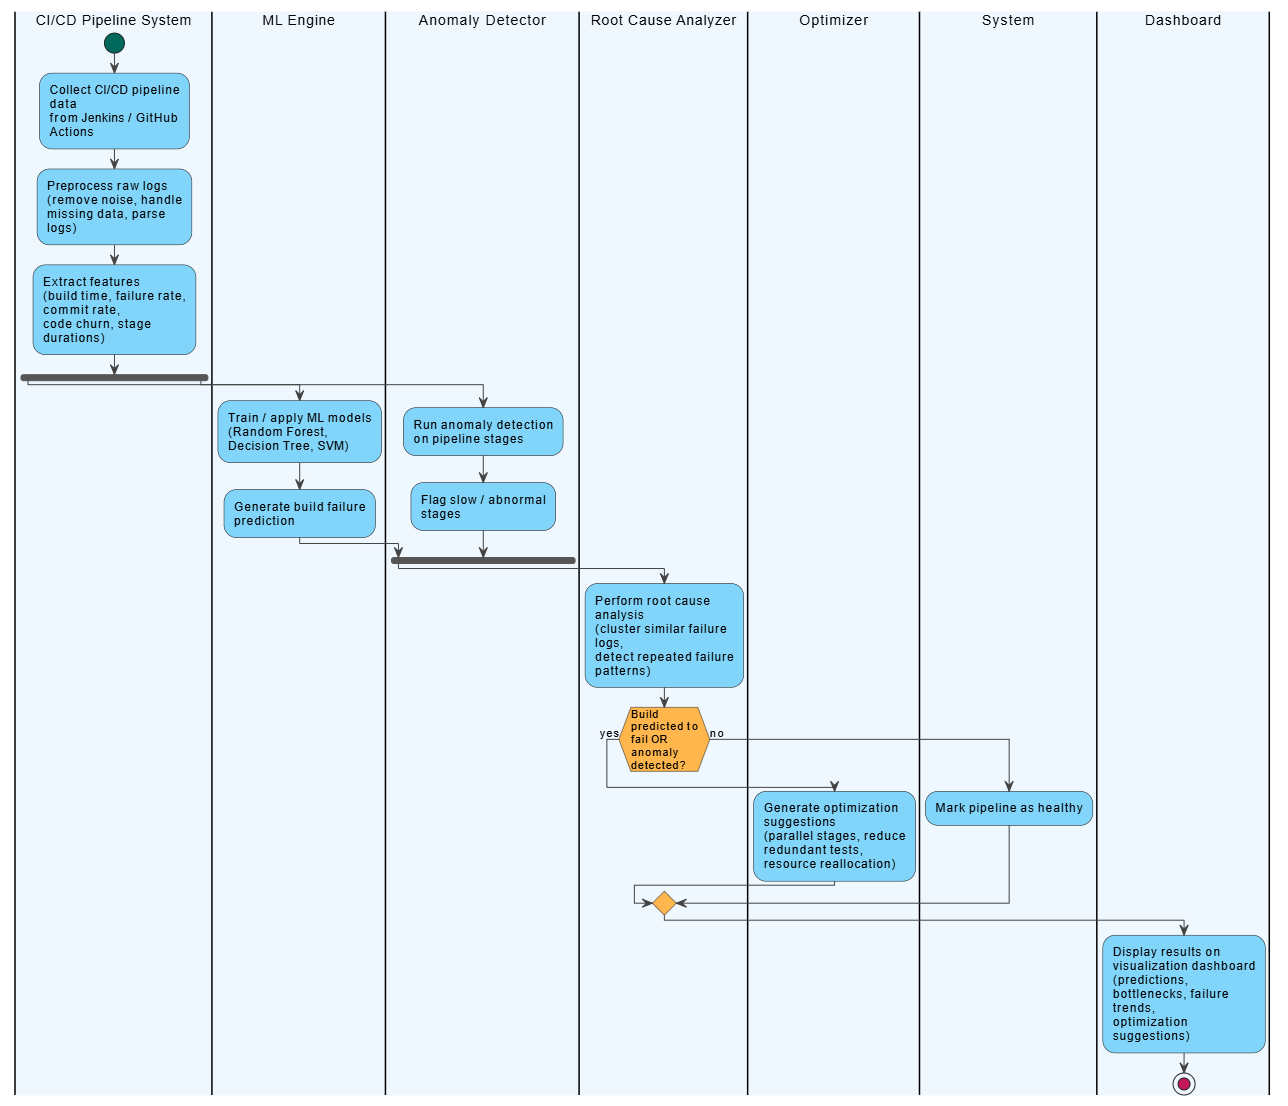
\includegraphics[width=\textwidth]{fig_activity.png}
\caption{Activity diagram of the CI/CD optimization system}
\label{fig:activity}
\end{figure}
The activity diagram depicts the flow of events in the system (Fig~\ref{fig:activity}).
\begin{enumerate}
\item CI/CD pipeline data is gathered from repositories and build systems.
\item The data is preprocessed and passed to feature engineering.
\item Machine learning models produce build failure predictions. In the deployed system this happens when a GitHub Actions run is requested, before it executes.
\item The anomaly detection and root cause analysis components detect bottlenecks and recurring failure patterns.
\item When a build is predicted to fail or an anomaly is found, optimization suggestions are generated.
\item Finally, the results are displayed on the dashboard.
\end{enumerate}

\subsection{Use Case Diagram}
\label{sec:usecase}
\begin{figure}[H]
\centering
\begin{tikzpicture}[
  font=\small,
  uc/.style={draw, ellipse, align=center, minimum width=52mm, minimum height=10mm, inner sep=1pt, fill=white},
  actor/.style={align=center, font=\small},
  link/.style={thick}]
\node[draw, thick, rounded corners=3pt, minimum width=84mm, minimum height=138mm, label={[font=\small\bfseries]above:AI-Driven CI/CD Optimization System}] (sys) at (0,0) {};
\foreach \name/\y/\txt in {u1/6.0/{View dashboard, trends\\and model evidence}, u2/4.3/{View pipeline risk timeline\\and alerts}, u3/2.6/{Submit build for scoring}, u4/0.9/{Explore what-if scenarios}, u5/-0.8/{Download build report}, u6/-2.5/{View failure diagnosis\\and suggestions}, u7/-4.2/{Score requested workflow run}, u8/-5.9/{Record outcome, job telemetry\\and failed-job logs}}
  \node[uc] (\name) at (0,\y) {\txt};
\newcommand{\stick}{\tikz{\draw (0,0.45) circle (0.16); \draw (0,0.29) -- (0,-0.1); \draw (-0.22,0.18) -- (0.22,0.18); \draw (0,-0.1) -- (-0.18,-0.4); \draw (0,-0.1) -- (0.18,-0.4);}}
\node[actor] (dev) at (-6.6,1.7) {\stick\\Developer};
\node[actor] (gh) at (6.6,-3.6) {\stick\\GitHub Actions\\(webhooks)};
\node[actor] (col) at (6.6,-7.2) {\stick\\CI log collector};
\foreach \u in {u1,u2,u3,u4,u5,u6} \draw[link] (dev) -- (\u.west);
\draw[link] (gh) -- (u7.east);
\draw[link] (gh) -- (u8.east);
\draw[link] (col) -- (u8.south east);
\end{tikzpicture}
\caption{Use case diagram of the CI/CD optimization system}
\label{fig:usecase}
\end{figure}

The use case diagram (Fig~\ref{fig:usecase}) shows how users and external systems interact with the solution.

\minorhead{Actors}
\begin{itemize}
\item \textbf{Developer:} views the dashboard, pipelines and alerts, scores builds and explores what-if scenarios.
\item \textbf{GitHub Actions:} sends signed workflow-run and job events.
\item \textbf{CI log collector:} an optional workflow that uploads failed-job logs.
\end{itemize}

\minorhead{Use Cases}
\begin{itemize}
\item View dashboard, failure trends and model evidence
\item View a pipeline's risk timeline and alerts
\item Submit a build for scoring
\item Explore what-if scenarios
\item Download a per-build PDF report
\item View failure diagnosis and optimization suggestions
\item Score a requested workflow run automatically
\item Record run outcomes, job telemetry and failed-job logs
\end{itemize}
